\documentclass[tikz]{standalone}
\begin{document}

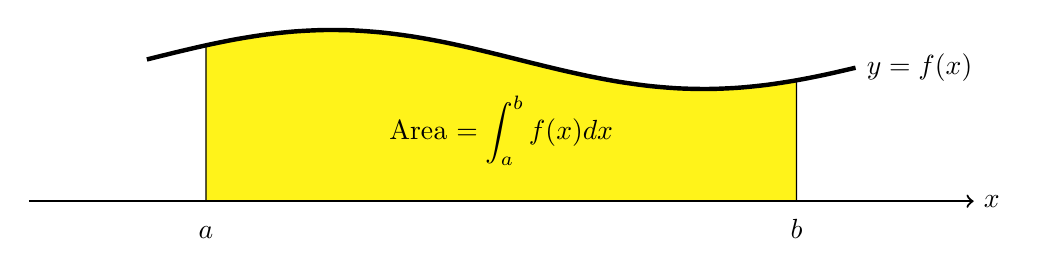
\begin{tikzpicture}[scale=1.5]

  % shade region
  \draw[fill=yellow!90,domain=0.5:5.5,smooth,variable=\x] (0.5,0) -- plot ({\x},{1.2 + 0.25*sin(\x r)}) |- cycle;

  % draw axis
  \draw[thick,->] (-1,0) -- (7,0) node[right] {$x$};

  % draw curve
  \draw[ultra thick,domain=0:6,smooth,variable=\x,black] plot ({\x},{1.2 + 0.25*sin(\x r)}) node[right]{$y=f(x)$};

  \node at (0.5, -0.4) [above] {$a$};
  \node at (5.5, -0.4) [above] {$b$};      
        
  \node at (3, 0.6) {Area $ = \displaystyle \int_a^b f(x)dx$};
\end{tikzpicture}
\end{document} 
